% =========================================================================
% PPCF draft (single column). Structure: A problem (weak edge-side CES) -> B what sets
% the limit (regime number; its dependence on radius on MAST and across KSTAR
% discharges) -> C what the CES past alone leaves -> D what co-located fast diagnostics
% add on KSTAR -> E character of the gain.
% Numbers: docs/paper/short/main_short.tex (KSTAR, traced there to the frozen
% artifacts), docs/paper/review_loop/analyses/{R2,R3}/*.json, docs/paper/mast_gate.json,
% docs/paper/mast_gate_addendum1.json, docs/paper/mast_gate_addendum2.json,
% docs/paper/b29_causal.json, docs/paper/ppcf/kstar_regime.json, kstar_level.json.
% Check: py docs/paper/ppcf/check_numbers.py
% Build (from this folder): latexmk -pdf main_ppcf
% =========================================================================
\documentclass[11pt,a4paper]{article}

\usepackage[margin=2.6cm]{geometry}
\usepackage[T1]{fontenc}
\usepackage[utf8]{inputenc}
\usepackage{newtxtext,newtxmath}
\usepackage{amsmath,bm}
\usepackage{graphicx}
\usepackage{booktabs}
\usepackage{multirow}
\usepackage[skip=6pt]{caption}
\usepackage{microtype}
\usepackage[numbers,sort&compress]{natbib}
\usepackage[colorlinks=true,linkcolor=blue,citecolor=blue,urlcolor=blue]{hyperref}

\newcommand{\Ti}{\ensuremath{T_i}}
\newcommand{\Vrot}{\ensuremath{V_\mathrm{rot}}}
\newcommand{\Vi}{\ensuremath{V_i}}
\newcommand{\chir}{\ensuremath{\chi^2_\mathrm{red}}}

\hypersetup{
  pdftitle={Estimating charge-exchange ion temperature and rotation without the next measurement: a fit-noise-limited edge chord on KSTAR and its radial counterpart on MAST},
  pdfauthor={Seungsang Lee},
}

\title{Estimating charge-exchange ion temperature and rotation without the next
measurement: a fit-noise-limited edge chord on KSTAR and its radial counterpart on
MAST}
\author{Seungsang Lee\\
  {\small Department of Nuclear Engineering, Seoul National University, Seoul, Republic of Korea}\\
  {\small\texttt{lss010330@snu.ac.kr}}}
\date{}

\begin{document}
\maketitle

% =========================================================================
\begin{abstract}
\noindent
Charge-exchange spectroscopy (CES) gives ion temperature \Ti{} and toroidal rotation
at 10\,ms on KSTAR. On an edge-side chord, where the signal is weak, 8.2\% of \Ti{} and
23.9\% of rotation samples are missing. We ask what limits an
estimate that cannot wait for the next CES sample. The lag-1 autocorrelation of 10\,ms
increments is $-0.416$ $[-0.429, -0.402]$ for \Ti{} on KSTAR (fit-noise-limited). On 88 public MAST discharges it is $+0.297$ $[+0.197, +0.352]$
pooled over radius, but $+0.103$ $[-0.079, +0.257]$ at the normalized radius of the
KSTAR chord, where 43\% of samples fail the fit rule against 23\% in the core. The
main result is on
KSTAR: among estimators that do not use the next CES sample, a recurrent network that
also reads co-located beam-emission and electron-cyclotron channels has the lowest \Ti{} mean squared error, with skill $+0.113$ $[+0.085, +0.132]$ over a
CES-only causal Gaussian process, and $+0.059$ to $+0.117$ over the same network
retrained without them when failed fits are excluded. Against an offline
Gaussian
process the interval includes zero. Rotation is estimated from its own history
(fast-channel coupling $|r| \leq 0.044$), with skill $+0.265$ $[+0.198, +0.326]$ over
persistence. The gain is carried by large-error rows.
\end{abstract}

% =========================================================================
\section{Introduction}
\label{sec:intro}

Ion temperature \Ti{} and toroidal rotation \Vrot{} enter every account of core
confinement, momentum transport and stability in a tokamak. Both are measured by
charge-exchange spectroscopy (CES)~\citep{Ko2010ChargeExchange}, which infers \Ti{}
from the Doppler broadening and \Vrot{} from the Doppler shift of a charge-exchange
line excited by a neutral beam. The measurement integrates photons over an exposure and
then fits a line shape, so it is slower than most other core diagnostics and it fails
intermittently. It fails most where the signal is weakest. The KSTAR chord used here
is on the edge side of the plasma, towards the pedestal (nominal normalized radius
about 0.8; the median \Ti{} per discharge is 528\,eV), where the charge-exchange
emission is low, exposures more often return no value and line fits more often fail.
On the 10\,ms grid of the KSTAR data used here, 8.2\% of \Ti{} samples
and 23.9\% of \Vrot{} samples are missing at one chord, independently of each other,
and the missing rate is not random: it rises from 0.77\% to 4.45\% across quintiles of
the neighbouring-step change and is 19.9\% in the lowest quintile of beam-emission
intensity against 3.7\% in the highest~\citep{Little2002StatisticalAnalysis}. Meanwhile
beam-emission spectroscopy (BES), electron-cyclotron-emission imaging (ECEI) and Mirnov
coils observe the same plasma without gaps, but none of them measures \Ti{} or \Vrot{}.

Two kinds of estimate can fill such a sample. An \emph{offline} estimate may use the
CES samples on both sides and is appropriate for post-discharge analysis. An estimate
that \emph{does not use the next CES sample} is the one a monitoring or control
application needs, because the next exposure may be 10\,ms away or may not arrive at
all. This paper is about the second kind. The question is physical before it is
statistical: what, in the plasma and in the measurement, sets how well a missing CES
sample can be estimated from what is available at that time?

\paragraph{Line of argument.}
The paper follows one chain. (A) CES leaves gaps that are not at random
(\S\ref{sec:data}), on a chord where the measurement is weak. (B) How well a gap can
be filled is set first by whether successive CES increments are dominated by fit noise
or by plasma evolution; one number, the lag-1 autocorrelation of 10\,ms increments,
measures this. The KSTAR chord is fit-noise-limited. On MAST, which has many chords,
the number is positive in the core, the measurement weakens outward of a normalized
radius of 0.7, and at the radius of the KSTAR chord the number is no longer separated
from zero; inside KSTAR the same number orders the simple estimators from discharge to
discharge (\S\ref{sec:regime}). (C) Where per-sample fit errors are available (MAST),
the best estimator that reads only the CES past still leaves a residual above the
reported fit noise in two of four campaigns for \Ti{} and in all four for rotation, so
information outside the CES history has room to act (\S\ref{sec:floor}). (D) On KSTAR,
where fast diagnostics view the same location as the CES chord, an estimator that
reads them has a lower \Ti{} error than every CES-only estimator that does not use the
next sample, and the same network retrained without them has a larger error when
failed fits are excluded; for rotation the same channels carry a bounded, small
association, and the estimate comes from the rotation history alone
(\S\ref{sec:fast}). (E) The gain is a property of the large-error rows, not of
the typical row, and a 20-parameter filter read from the network reproduces most of it
(\S\ref{sec:character}). The headline result is link (D) for \Ti{}: among estimators
that do not use the next CES sample, the full-input estimator has the lowest mean
squared error, with skill $+0.113$ $[+0.085, +0.132]$ over the CES-only causal GP.

\paragraph{Scope of the statements.}
The KSTAR result is one chord, one campaign and one device. MAST enters as a second,
public device for links (B) and (C) only: it has many chords and per-sample fit errors,
which KSTAR files lack, but no fast diagnostic co-located with the CES chords, so no
MAST number is used as support for link (D). The two devices pose different problems
(natural gaps at 10\,ms on KSTAR, frames hidden by us at 5\,ms on MAST), the pooled
MAST numbers are not at the radius of the KSTAR chord, and the comparison is not a
replication. The breakdowns of the MAST result by radius and by campaign were made
after the pooled result had been seen and are labelled post hoc. For link (D) the
fast-channel share of the \Ti{} margin is measured with a retrained network; it holds
in the population that excludes failed fits and carries one open check on training
length (\S\ref{sec:limits}). The equilibrium of the KSTAR discharges is not in the
files, so the position of the chord relative to the pedestal is not established
discharge by discharge, and no statement about pedestal dynamics is made.

% =========================================================================
\section{Related work}
\label{sec:related}

\paragraph{Profile fitting and interpolation.} Gaussian-process (GP)
regression~\citep{rasmussen2006} is the standard tool for fusion profile
fitting~\citep{chilenski2015,michoski2024} and has been applied to KSTAR CES \Ti{}
profiles~\citep{Kim2024KineticProfile}; PCHIP~\citep{fritsch1980} avoids spline ringing
at steps. Persistence as a reference has precedent in fusion profile
forecasting~\citep{Abbate2025Combining} and space weather~\citep{Owens2013Persistence};
skill is scored after Murphy~\citep{murphy1988}.

\paragraph{Neural inference of ion quantities.} A neural network that extracts \Ti{}
and rotation from KSTAR CES spectra without beam
modulation~\citep{Lee2026NeuralNetworkbased} is the closest prior work: it reads a
spectrum that exists, whereas the present problem is the grid time at which no usable
CES value exists. The KSTAR files do not record whether a missing value had no exposure
or a rejected fit, so the share of each case is not measured. Lin et
al.~\citep{Lin2024PredictionPlasma} map an x-ray crystal spectrometer to \Ti{} and
rotation on EAST, an instantaneous mapping within one photon channel.
RTCAKENN~\citep{Shousha2023MachineLearningbased} reconstructs kinetic profiles in real
time and tolerates dropped inputs; there missingness is a robustness condition, here
the sparsity of the target itself is the problem.

\paragraph{Cross-diagnostic reconstruction.} Diag2Diag synthesizes Thomson
$T_e$ and $n_e$ from simultaneous diagnostics on
DIII-D~\citep{Jalalvand2025MultimodalSuperresolution} with a memoryless network; related
work densifies Thomson scattering on COMPASS~\citep{Imrek2026TemporalSuperresolution},
fills Thomson intervals with an extended Kalman filter on
TCV~\citep{Pastore2023ModelBased}, restores EAST $T_e$ and
$Z_\mathrm{eff}$~\citep{Wang2025TimeSeries,Jia2026TimeSeries} and masks channels on
HL-3~\citep{Yang2026FusionmaeSelfsupervised}. These target electron or generic dense
channels. The present work extends that programme to a sparse ion channel, to
estimation conditioned on the irregular past of the target itself, and to a per-target
test of whether the fast channels are informative at all.

\paragraph{Methods used.} Observation masks follow
GRU-D~\citep{Che2018RecurrentNeural}; the overlap-corrected cross-validation interval
is that of Nadeau and Bengio~\citep{Nadeau2003Inference}; the repeat-then-discharge
resampling is a hierarchical bootstrap~\citep{Saravanan2020Hierarchical}; reading a
recurrent network through its input--output response
follows~\citep{Maheswaranathan2020HowRecurrent}.

% =========================================================================
\section{Data}
\label{sec:data}

\subsection{KSTAR}
\label{sec:data:kstar}
We use 641 KSTAR discharge files of the 2022 campaign (shots 30801--32751) aligned to a
10\,ms grid, 247{,}207 rows in total. Each row holds nine BES
channels~\citep{Nam2012AnalysisEdge}, four ECEI
channels~\citep{Yun2010DevelopmentKstar}, two Mirnov-coil signals, time, and the two
CES targets, which come from one outboard chord at $R = 2.198$\,m. No equilibrium is
in the files, so $r/a$ is not mapped; with the nominal major and minor radii (1.8 and
0.5\,m) the chord is at a normalized radius of $(2.198 - 1.8)/0.5 = 0.80$, and we refer
to it as an edge-side chord. The level of the measurement agrees with that position:
the median \Ti{} per discharge is 528\,eV (10th to 90th percentile 213 to 1{,}020\,eV
over 603 discharges). The BES and ECEI channels lie within about 1.5\,cm of that chord; the
two Mirnov inputs are two positions of one poloidal array. \Ti{} is missing in 8.2\% of
rows and \Vrot{} in 23.9\% (Fig.~\ref{fig:missing}a). Rows group into contiguous
segments at breaks of at least 0.5\,s, and no estimator bridges such a break. Inside a
segment most gaps are short: the median gap is one row (10\,ms) for both targets, and
92.9\% of \Ti{} gaps and 89.8\% of \Vrot{} gaps are 50\,ms or shorter
(Fig.~\ref{fig:missing}b).

\begin{figure}[t]
  \centering
  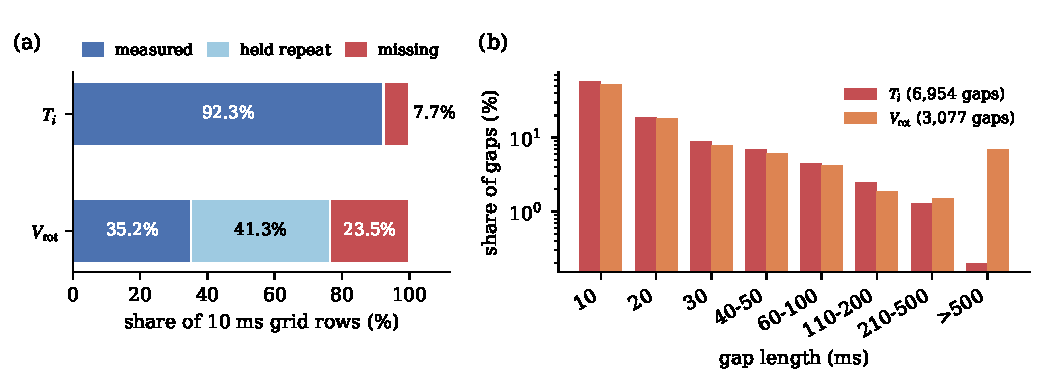
\includegraphics[width=\linewidth]{fig_missing}
  \caption{CES missingness on the KSTAR 10\,ms grid (641 discharges, 247{,}207 rows).
  (a) Share of grid rows per target that carry an independent measurement, a held
  repeat of the previous value, or no value. \Ti{} and \Vrot{} go missing independently
  (8.2\% and 23.9\%); counting held values, 65.0\% of the grid carries no independent
  \Vrot{} measurement. (b) Lengths of the gaps (runs of consecutive rows without a
  value inside a contiguous segment), as a share of the 8{,}233 \Ti{} gaps and 4{,}351
  \Vrot{} gaps; logarithmic vertical axis.}
  \label{fig:missing}
\end{figure}

\paragraph{Held rotation values.} 54\% of the observed \Vrot{} values repeat the
previous observation bit for bit (runs of up to 1{,}214 rows, in 499 of 641 files), so
only 35.0\% of the grid carries an independent \Vrot{} measurement; \Ti{} has one such
row in 226{,}991. The files do not record why. Held values are removed everywhere,
from targets, history inputs, normalization statistics and the anchors of every
reference estimator, so that no estimator is credited for repeating a held value.

\paragraph{Fit failures and two populations.} 1{,}197 \Ti{} rows (0.53\%) exceed
3\,keV; they are isolated (951 runs in 274 discharges, 85\% of runs single rows) and
are failed line fits. Because they also corrupt the anchors of every interpolant, all
KSTAR results are given in two co-primary populations fixed in advance: \emph{cut}, in
which values above 3\,keV are treated as missing for every estimator, and
\emph{inclusive}, in which they are kept. The threshold is immaterial between 2.5 and
4\,keV (mean \Ti{} skill over PCHIP $+0.230$ and $+0.232$ against $+0.236$ at 3\,keV).
For rotation, a further scoring rule drops the rows whose target or anchor exceeds
$|\Vrot| = 1{,}000$\,km/s; it was set after the influence of those rows was known and
is discussed where it is used (\S\ref{sec:fast:vrot}).

\subsection{MAST}
\label{sec:data:mast}
The second device enters through the public FAIR-MAST
archive~\citep{Jackson2024FairMast} (licence CC BY-SA 4.0), level-1 source of the
time-resolved charge-exchange system~\citep{Conway2006HighThroughput}: \Ti{}, toroidal
velocity \Vi{} and their reported fit errors on up to 96 or 160 stored chord columns at
5\,ms frames. Campaigns M6--M9 span shots 14708--30473 (2006--2013); the catalogue
lists a conventional divertor for every shot used here. Of the 7{,}970 shots of these
campaigns that list this source, 13 had been inspected
in a pilot and were excluded; from the remaining 7{,}957 a list of 300 shots (75 per
campaign, catalogue quality flag ``Not Checked'') was drawn with a fixed seed from the
catalogue alone. 264 of the 300 carry the arrays and 261 have 5\,ms frames; the 17
listed shots tagged as heated by the south-west beam alone are all among the 36
without arrays. Within each
campaign, shots alternate between a tuning set (133 shots) and a test set (131 shots);
hyperparameters are chosen on the tuning set and every MAST number below is from the
test set.

A sample is a \emph{good fit} if \Ti{} is finite and positive, below 5\,keV, with a
positive reported error and a relative error below 0.1 (population G, primary) or below
0.5 (population W). The \emph{beam block} of a shot is the span from the first to the
last frame with at least ten good chords (at least 20 frames); a chord is scored if it
is good in at least 90\% of the block. In population G, 169 of the 261 shots have a
block and scored chords; the median block is 57 frames (0.29\,s), and the test set
holds 58{,}844 scored rows from 88 shots. Inside a block almost every frame is
measured, so MAST has no counterpart of KSTAR's natural gaps: we hide every second
frame of the block and estimate it from the visible frames of the same chord, which
are then 10\,ms apart. The frame times stored for a few shots are irregular or
non-increasing (4 shots in population G); the estimators therefore use the nominal
5\,ms grid, and dropping those shots changes no statement.

For the comparison with the KSTAR chord, each MAST chord is assigned a normalized
radius $\rho = (R - R_\mathrm{axis})/(R_\mathrm{out} - R_\mathrm{axis})$ from the
magnetic-axis and outer-boundary radii of the catalogue (one pair per discharge,
available for 122 of the 131 test shots; low-field side only), in the bins 0--0.3,
0.3--0.5, 0.5--0.7, 0.7--0.9 and 0.9--1.0. The bin 0.7--0.9 contains the nominal
radius of the KSTAR chord. The bins were fixed before the binned values were computed,
but after the pooled MAST result was known.

% =========================================================================
\section{Estimators and evaluation}
\label{sec:methods}

\subsection{Estimators that read only the CES series}
\label{sec:methods:ces}
Four estimators use the CES past of the target and nothing else: \emph{persistence}
(the last observed value), a \emph{running mean} (an exponentially weighted mean of
past observations, its constant chosen on validation data), a \emph{slope-state
filter} (a Kalman filter with level and slope states; MAST only) and a \emph{causal
GP} (Mat\'ern-3/2 kernel on the most recent past samples: 16 on KSTAR with per-sample
marginal-likelihood selection, 8 on MAST with hyperparameters tuned on the tuning
set). Three estimators also use the following CES sample and serve as offline
references: linear and PCHIP interpolation and an \emph{offline GP} with neighbours on
both sides. Where no later neighbour exists the interpolants return persistence (0.2\%
of scored \Ti{} rows and 0.3--0.5\% of scored \Vrot{} rows on KSTAR).

\subsection{A two-branch recurrent estimator for KSTAR}
\label{sec:methods:net}
Ion energy and toroidal angular momentum obey
\begin{align}
  \partial_t\bigl(\tfrac{3}{2}n_i T_i\bigr) + \nabla\!\cdot\!\mathbf{q}_i
    &= Q_{ei}\,(T_e-T_i) + S_i,
  \label{eq:energy}\\
  \partial_t\bigl(n_i m_i \langle R^2\rangle \omega_\varphi\bigr)
    + \nabla\!\cdot\!\Pi_\varphi
    &= T_\mathrm{NBI} + T_\mathrm{NTV} + T_\mathrm{int} + \cdots .
  \label{eq:momentum}
\end{align}
Both constrain a rate. BES responds to density and ECEI to electron temperature at the
location of the CES chord, the quantities that appear in the exchange and flux terms
of~\eqref{eq:energy}. None of the available channels measures a term
of~\eqref{eq:momentum}: there is no torque or beam-power signal, a Mirnov $dB/dt$ signal
sampled at 100\,Hz cannot see a static perturbation or resolve kHz mode rotation, and
BES intensity is not the momentum flux. The expectation from the equations is therefore
asymmetric, and the estimator is wired accordingly (Fig.~\ref{fig:arch}): the \Ti{}
branch reads the 15 fast channels and the CES past; the \Vrot{} branch reads the CES
past only. The asymmetry is then tested as a measurement in \S\ref{sec:fast:vrot}
rather than assumed.

\begin{figure}[t]
  \centering
  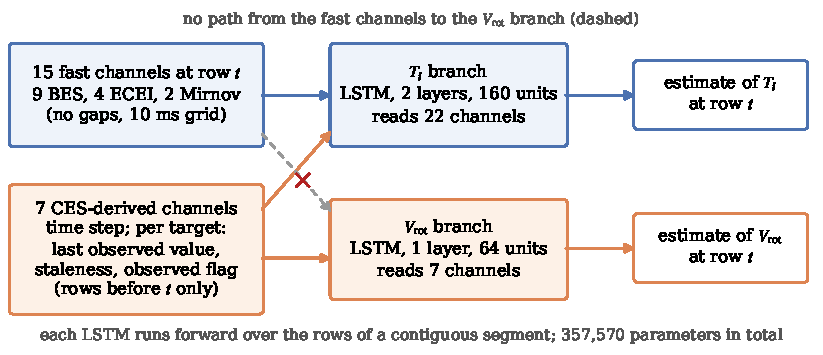
\includegraphics[width=0.9\linewidth]{fig_arch}
  \caption{The two-branch recurrent estimator for one KSTAR grid row $t$. 22 inputs
  (15 fast channels; time step; per target the last observed value, its staleness and
  an observed flag) feed two LSTMs that run forward in time. The \Ti{} branch reads all
  22 (2 layers, 160 units), the \Vrot{} branch only the seven CES-derived channels (1
  layer, 64 units). The dashed path from the fast channels to the \Vrot{} branch does
  not exist by construction. 357{,}570 parameters.}
  \label{fig:arch}
\end{figure}

At grid time $t$ the network estimates the normalized $y_t=[\Ti,\Vrot]_t$ with
per-target observation masks $m_{t,c}\in\{0,1\}$ and the loss
\begin{equation}
  \mathcal{L}
  = \frac{\sum_{t,c} m_{t,c}\,(\hat y_{t,c}-y_{t,c})^2}{\sum_{t,c} m_{t,c}}
  + \lambda\,\overline{\mathrm{ReLU}(z_0-\hat y_{t,\Ti})},\qquad \lambda = 0.1,
  \label{eq:loss}
\end{equation}
whose first term is minimized by the conditional mean; the second discourages \Ti{}
below the normalized zero $z_0$. A row with one observed target still supervises it.
The network keeps every input-complete row of a contiguous segment as context, since
the fast diagnostics have no gaps. The CES-derived inputs at $t$ use rows before $t$
only, and the target row never enters the input. Training uses AdamW (learning rate
$10^{-3}$, weight decay $10^{-4}$, batches of 16 segments, gradient clipping at 1.0,
early stopping with a 30-epoch cap); splits are by whole discharge file.

\paragraph{What is and is not causal.} The recurrent operator runs forward in time,
but the 15 fast channels are standardized with the mean and variance of the whole
discharge, which is an offline step. The estimator is therefore described as one that
\emph{does not use the next CES sample}, not as a causal estimator. A variant with a
standardizer that uses only past rows is not reported here (\S\ref{sec:limits}). A stateful step costs 0.97\,ms (median) and 1.49\,ms (99th
percentile) on a CPU.

\subsection{Scoring, intervals and registration}
\label{sec:methods:eval}
Errors are computed per target in physical units on rows where the target was measured
and withheld from the estimator; every estimator is scored on the identical set of
rows. The score is the mean-squared-error skill of estimator $A$ against a reference
$R$, $1 - \mathrm{MSE}_A/\mathrm{MSE}_R$ (zero means equal error). A result is given as
a point estimate, a 95\% interval and whether the interval excludes zero.

\paragraph{KSTAR.} The primary readout is \emph{pooled}: shot-level 5-fold
cross-validation on 639 discharges is repeated over eight re-partitions; in each
repeat the five test folds are concatenated into one skill, and a two-level bootstrap
draws a repeat and then resamples its discharges. This interval conditions on the
trained models and does not carry the correlation between overlapping training sets.
Two secondary readouts are given beside it: four file-level splits, each with its own
shot-clustered bootstrap interval (10{,}000 resamples) and the count of splits whose
interval excludes zero~\citep{Weissgerber2015Beyond,Agarwal2021Deep}; and the
fold-level interval of Nadeau and Bengio over 50 folds, which does carry the overlap
correlation. On the first of the four splits the test set holds 32{,}589 \Ti{} rows
over 96 shots and 10{,}463 \Vrot{} rows over 60 shots (cut).

\paragraph{MAST.} Intervals are from 2{,}000 bootstrap resamples of test shots, with
the same resample indices for every estimator. Besides the skill, each residual is
compared with the fit noise: the reduced chi-square \chir{} is the squared residual
divided by the variance that the reported errors alone predict for that estimator,
$\sigma_t^2 + \sum_i w_i^2\sigma_i^2$, where $w_i$ are the weights the (linear)
estimator puts on the visible samples. A residual that is fit noise only gives a mean
of 1 and, for Gaussian errors, a median of 0.455.

\paragraph{Registration and disclosures.} For each batch of runs the hypotheses,
decision rules and numerical expectations were committed to the public repository
before the batch was run; there is no third-party registry. On KSTAR, test files were
reserved before the architecture was chosen, but the adoption of the full-grid
recurrent design and of per-discharge standardization used results on the same four
test splits, and the repeated cross-validation re-partitions the same discharges. On
MAST, the shot list, the fit rule, the tuning/test division, the estimators and both
decision rules were committed before any value of the 300 shots was read. The tuning
grids of that first registered run placed several optima on a grid edge, so a second
run with wider grids was registered; the main text reports the second run, and the
first run, which leads to the same two decisions, is in
Appendix~\ref{app:mastfirst}. The order of events, including two execution defects
that were found and corrected, is given in Appendix~\ref{app:registration}.

% =========================================================================
\section{What sets the limit: the regime of the increments and its dependence on radius}
\label{sec:regime}

Let $y_t$ be the CES series on a chord and $d_t = y_t - y_{t-1}$ its 10\,ms increment.
If the plasma value is constant over a few samples and each sample carries independent
fit noise, successive increments share one noise term with opposite sign and their
correlation is $-0.5$. If the plasma value evolves smoothly and the noise is small,
successive increments have the same sign and the correlation is positive. The lag-1
autocorrelation of increments is therefore a \emph{regime number}: it says whether the
last CES sample differs from the next one mostly because of the fit or mostly because
of the plasma.

\begin{figure}[t]
  \centering
  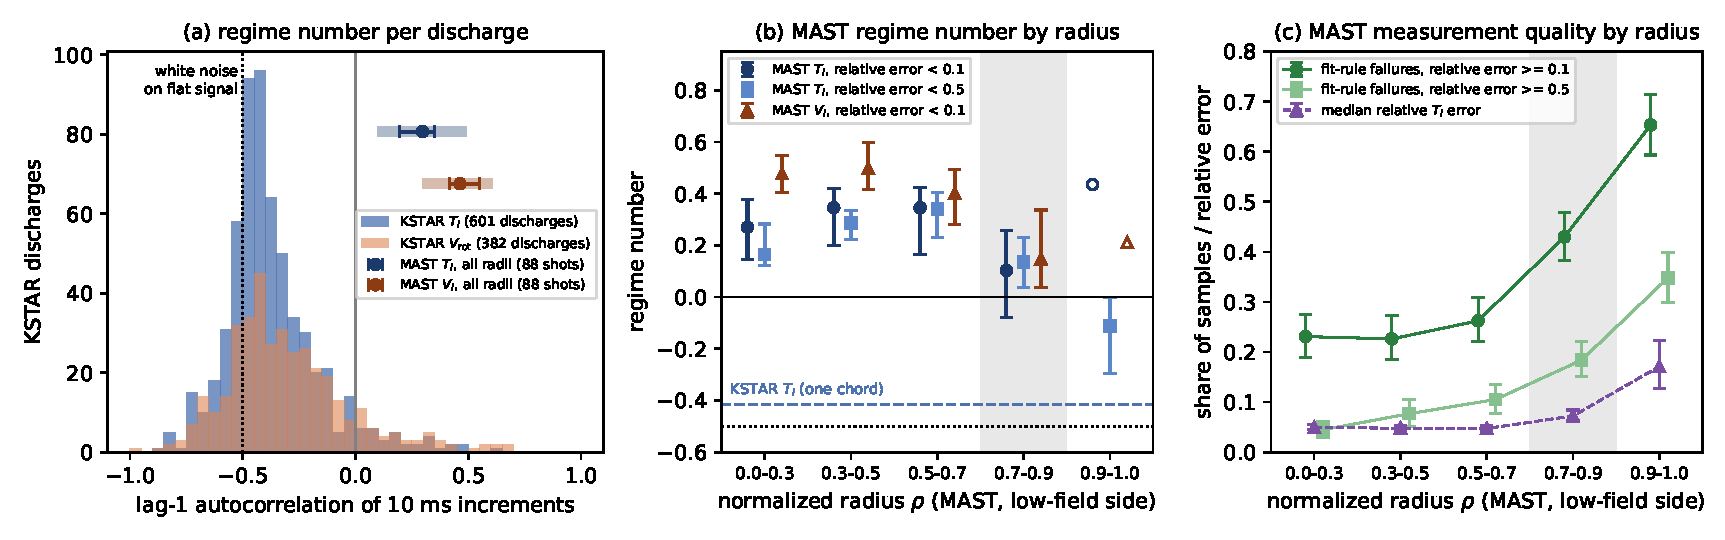
\includegraphics[width=\linewidth]{fig_regime}
  \caption{The regime number. (a) Lag-1 autocorrelation of 10\,ms increments per
  discharge. Histograms: KSTAR \Ti{} (cut) and \Vrot{} (held values removed), one
  edge-side chord. Markers: MAST \Ti{} and \Vi{} on the visible (10\,ms) series, all
  scored chords pooled, median over 88 test shots with 95\% interval; the shaded bar
  is the interquartile range. The dotted line is the value for white noise on a flat
  signal. (b) MAST regime number by bin of normalized radius (post hoc breakdown),
  median over test shots with 95\% interval, for \Ti{} under the two fit rules and for
  \Vi{}; open markers are bins with fewer than eight shots. The grey band is the bin
  that contains the nominal radius of the KSTAR chord and the dashed line is the KSTAR
  \Ti{} value. (c) MAST measurement quality by the same bins, before the fit rule is
  applied: share of samples failing the rule and median relative \Ti{} error.}
  \label{fig:regime}
\end{figure}

\begin{table}[t]
  \centering
  \caption{Regime number (lag-1 autocorrelation of 10\,ms increments): median over
  discharges with 95\% interval, and interquartile range. KSTAR: per discharge over
  triples of consecutive measured rows, \Ti{} in the cut population and \Vrot{} with
  held values removed, one edge-side chord. MAST: visible (10\,ms) series of the test
  shots, population G, all scored chords pooled (Table~\ref{tab:radius} resolves the
  radius). White noise on a flat signal gives $-0.5$.}
  \label{tab:regime}
  \footnotesize
  \begin{tabular}{llccc}
    \toprule
    Device & Target & Discharges & Regime number & Interquartile range \\
    \midrule
    KSTAR & \Ti{} & 601 & $-0.416$ $[-0.429, -0.402]$ & $-0.491$ to $-0.294$ \\
    KSTAR & \Vrot{} & 382 & $-0.349$ $[-0.384, -0.322]$ & -- \\
    MAST & \Ti{} & 88 & $+0.297$ $[+0.197, +0.352]$ & $+0.096$ to $+0.493$ \\
    MAST & \Vi{} & 88 & $+0.463$ $[+0.416, +0.549]$ & $+0.298$ to $+0.606$ \\
    \bottomrule
  \end{tabular}
\end{table}

\paragraph{The KSTAR chord is fit-noise-limited.} The regime numbers of \Ti{} and \Vrot{} on KSTAR
sit close to the white-noise value (Table~\ref{tab:regime},
Fig.~\ref{fig:regime}a). This is a
descriptive statistic computed for this paper, not a registered test. It agrees with
two independent readings of the same data: difference estimators put the \Ti{}
measurement noise at 46.4--129.9\,eV, the order of the best estimator's error
(157.8\,eV), and the ratio of the relative 10\,ms scatter of \Ti{} to that of \Vrot{}
is $\sqrt2$ (1.395--1.532 in eight split--population cells), the value for independent
Gaussian line-fit errors on width and shift.

\paragraph{MAST, pooled over radius, is trend-limited.} On the visible 10\,ms series
of the MAST test shots the regime number is positive for both targets, with intervals
above zero (Table~\ref{tab:regime}). Beam blocks last about 0.3\,s and the plasma is
evolving during them, so successive increments point the same way. The sign does not
depend on the campaign or on the stored array layout: by campaign (M6 to M9) the \Ti{}
number is $+0.109$ $[+0.056, +0.337]$, $+0.226$ $[+0.101, +0.339]$, $+0.345$
$[+0.197, +0.595]$ and $+0.359$ $[+0.205, +0.497]$, and the \Vi{} number is $+0.383$,
$+0.419$, $+0.569$ and $+0.524$, every interval above zero; for the arrays stored with
160 and with 96 chord columns it is $+0.278$ $[+0.139, +0.384]$ and $+0.307$
$[+0.196, +0.386]$ for \Ti{}. These breakdowns were made after the pooled result was
known, the strata are confounded with each other, and no correction for the number of
strata is applied.

\begin{table}[t]
  \centering
  \caption{MAST test shots by bin of normalized radius $\rho$ (low-field side; post
  hoc breakdown, bins fixed before the binned values were computed). Columns 2--3:
  samples inside the beam block before the fit rule is applied (112 shots; 105 in the
  outermost bin), share failing the rule at a relative \Ti{} error of 0.1 and median
  relative \Ti{} error. Columns 4--6: regime number, median over shots with 95\%
  interval, with the number of shots; G and W are the fit rules at relative error 0.1
  and 0.5. The bin 0.7--0.9 contains the nominal radius of the KSTAR chord, whose
  \Ti{} regime number is $-0.416$. An entry without an interval has fewer than eight
  shots.}
  \label{tab:radius}
  \footnotesize
  \setlength{\tabcolsep}{3pt}
  \resizebox{\linewidth}{!}{%
  \begin{tabular}{lccccc}
    \toprule
    $\rho$ & Fail share & Rel.\ error & \Ti{}, G & \Ti{}, W & \Vi{}, G \\
    \midrule
    0--0.3 & 0.231 $[0.189, 0.276]$ & 0.050 & $+0.271$ $[+0.145, +0.379]$ (75) & $+0.165$ $[+0.121, +0.283]$ (105) & $+0.478$ $[+0.406, +0.546]$ \\
    0.3--0.5 & 0.226 $[0.185, 0.273]$ & 0.048 & $+0.346$ $[+0.198, +0.420]$ (66) & $+0.287$ $[+0.223, +0.335]$ (99) & $+0.499$ $[+0.416, +0.598]$ \\
    0.5--0.7 & 0.262 $[0.222, 0.308]$ & 0.047 & $+0.346$ $[+0.167, +0.424]$ (54) & $+0.341$ $[+0.230, +0.403]$ (93) & $+0.401$ $[+0.282, +0.495]$ \\
    0.7--0.9 & 0.430 $[0.384, 0.478]$ & 0.072 & $+0.103$ $[-0.079, +0.257]$ (26) & $+0.136$ $[+0.036, +0.230]$ (72) & $+0.147$ $[+0.038, +0.337]$ \\
    0.9--1.0 & 0.653 $[0.593, 0.715]$ & 0.171 & $+0.435$ (6) & $-0.112$ $[-0.296, -0.000]$ (29) & $+0.212$ (6) \\
    \bottomrule
  \end{tabular}}
\end{table}

\paragraph{The measurement weakens outward, and the regime number is not the same at
all radii.} The pooled MAST number is an average over chords from the core to the
edge, whereas the KSTAR number is from one edge-side chord, so the two are not a
like-for-like comparison. Table~\ref{tab:radius} and Fig.~\ref{fig:regime}b,c resolve
the MAST test shots by normalized radius. Inside $\rho = 0.7$ the share of samples
that fail the fit rule is flat (0.231, 0.226, 0.262); in the bin that contains the
KSTAR radius it is 0.430 $[0.384, 0.478]$ and in the outermost bin 0.653
$[0.593, 0.715]$, and the median relative \Ti{} error rises from 0.047--0.050 to 0.072
and 0.171. The edge-side measurement is the weak one on MAST as well. The \Ti{} regime
number is $+0.271$ to $+0.346$ in the three inner bins; in the bin of the KSTAR radius
it is $+0.103$ $[-0.079, +0.257]$ under the primary fit rule, an interval that
includes zero (26 shots), and $+0.136$ $[+0.036, +0.230]$ under the loose rule (72
shots); in the outermost bin under the loose rule it is $-0.112$ $[-0.296, -0.000]$
(29 shots; the primary rule leaves six shots there). For \Vi{} the matched bin gives
$+0.147$ $[+0.038, +0.337]$.

Two statements written down before these binned values were computed asked for a
monotone ordering in $\rho$ and did not hold in that form: the failure share is flat
inside $\rho = 0.7$ and rises only outside it, and the \Ti{} regime number rises to
mid-radius before it falls. The registered difference between the matched bin and the
innermost bin is $-0.029$ $[-0.185, +0.070]$ under the loose rule and $-0.167$
$[-0.377, +0.018]$ under the primary rule; both intervals include zero. What the
breakdown supports is therefore limited: at the radius of the KSTAR chord the MAST
\Ti{} increments are not shown to be trend-dominated under the primary rule, the
distance to the KSTAR value is smaller than in the pooled comparison, and it is not
removed ($-0.416$ lies below both matched-bin intervals). The two devices also differ
in exposure, chord geometry and block length, and the contrast is not attributed to a
single cause.

\paragraph{The regime decides the yardstick.} In the noise-limited regime, averaging
the CES past removes noise: on KSTAR a running mean has \Ti{} skill $+0.26$ to $+0.34$
over persistence on the four splits, the causal GP $+0.31$ to $+0.35$, and for \Vrot{}
the running mean has $+0.161$ $[+0.060, +0.244]$ (pooled, cut). In the trend-limited
regime, averaging lags the trend: on MAST the best running mean is the one with the
shortest memory offered, and its skill over persistence has an interval below zero
for both targets, in each of the four campaigns ($-0.003$ to $-0.030$), while
estimators that carry a slope or a kernel have positive skill (Table~\ref{tab:mast}).
Across MAST test shots the regime
number is correlated with the difference between slope-filter and running-mean skill
(Spearman $+0.423$ $[+0.205, +0.598]$ for \Ti{}, $+0.779$ $[+0.656, +0.870]$ for
\Vi{}; both intervals exclude zero). One statement registered for MAST did not hold:
the slope-state filter's \Ti{} skill over persistence, $+0.076$ $[-0.006, +0.148]$,
includes zero.

\begin{table}[t]
  \centering
  \caption{KSTAR, \Ti{}, cut population: discharges grouped by tertile of their regime
  number (280 discharges with at least 30 scored rows). Pooled mean-squared-error
  skill with discharge-clustered 95\% intervals; bold = interval excludes zero.}
  \label{tab:tertile}
  \footnotesize
  \setlength{\tabcolsep}{5pt}
  \begin{tabular}{lcccc}
    \toprule
    Regime number & Discharges & Causal GP over & Running mean over & Recurrent estimator \\
     & & running mean & persistence & over causal GP \\
    \midrule
    $-0.85$ to $-0.48$ & 93 & $-0.006$ $[-0.027, +0.016]$ & $\mathbf{+0.393}$ $[+0.375, +0.412]$ & $\mathbf{+0.096}$ $[+0.058, +0.133]$ \\
    $-0.48$ to $-0.37$ & 94 & $-0.023$ $[-0.047, +0.005]$ & $\mathbf{+0.311}$ $[+0.289, +0.333]$ & $\mathbf{+0.137}$ $[+0.104, +0.166]$ \\
    $-0.37$ to $+0.35$ & 93 & $\mathbf{+0.064}$ $[+0.017, +0.117]$ & $+0.087$ $[-0.012, +0.166]$ & $\mathbf{+0.132}$ $[+0.063, +0.183]$ \\
    \bottomrule
  \end{tabular}
\end{table}

\paragraph{The same number orders the estimators inside KSTAR.} If the regime number
decides the yardstick, it should do so from discharge to discharge on one device. This
was registered as a prediction for KSTAR after it had held on MAST and before the
per-discharge values were computed. Across 280 KSTAR discharges, the rank correlation
between the regime number of a discharge and the difference between causal-GP skill
and running-mean skill is $+0.338$ $[+0.213, +0.451]$ for \Ti{} (cut; $+0.375$
$[+0.262, +0.477]$ inclusive) and $+0.574$ $[+0.442, +0.680]$ for \Vrot{} (170
discharges); every interval excludes zero. By tertile (Table~\ref{tab:tertile}),
averaging gains $+0.393$ over persistence in the most noise-dominated third and
$+0.087$ $[-0.012, +0.166]$, an interval including zero, in the least noise-dominated
third, where the causal GP has skill $+0.064$ $[+0.017, +0.117]$ over the running
mean. A second prediction did not hold: the margin of the recurrent estimator over
the causal GP was expected to grow with the regime number, and its rank correlation
is $-0.081$ $[-0.207, +0.048]$ (cut), including zero; the margin excludes zero in all
three tertiles. Two limits apply. The regime number and the errors are computed from
the same rows of the same discharge, and persistence error shares the frame-to-frame
noise with the regime number by construction. And the range is narrow: 3.2\% of the
\Ti{} discharges and 9.4\% of the \Vrot{} discharges have a positive regime number,
so the relation is established inside the noise-dominated range only.

The practical consequence is that the reference against which a learned estimator
should be judged depends on the regime. On the KSTAR chord, PCHIP passes exactly
through noisy anchors, so any smoother of the CES past gains on it (the running mean
has $+0.05$ to $+0.17$ over PCHIP, interval excluding zero on 3 of 4 cut splits), and
the deciding CES-only comparison is the causal GP. On MAST pooled over radius the
running mean is no reference at all and persistence is hard to improve on without a
slope.

% =========================================================================
\section{What the CES past alone leaves}
\label{sec:floor}

\subsection{Is a hidden MAST frame an independent measurement?}
\label{sec:floor:indep}
Scoring a hidden frame against an estimate built from its neighbours is meaningful
only if the frame's fit noise is independent of theirs. This was tested without using
the reported errors. For spacings $k = 1, 2, 4$ frames, the robust variance $S_k$ of
the second difference $y_{t+k} - 2y_t + y_{t-k}$ (divided by 6) equals the noise
variance plus a signal term that grows with $k$. If the noise is white in time and the
signal term grows as $k^p$ with $p \geq 1$, then
\begin{equation}
  T_a = \frac{S_1 - S_2 + (S_4 - S_2)/2}{S_2} \;\geq\; 0 ,
  \label{eq:ta}
\end{equation}
whereas a positive noise correlation $\rho_1$ between adjacent frames lowers $T_a$ by
about $(4/3)\rho_1$. The decision rule fixed in advance was that independence is
rejected if the interval of the median $T_a$ over test shots lies below zero. It is
$+0.453$ $[+0.341, +0.565]$ for \Ti{} and $+0.642$ $[+0.208, +1.148]$ for \Vi{}: no
adjacent-frame noise correlation is detected. The test is one-sided and conservative,
since signal variation raises $T_a$, and it is a statement about the median shot (26\%
and 31\% of single shots have $T_a < 0$).

The same second differences, compared with the variance the reported errors predict,
say how well the errors are calibrated at the median row: the ratio to the Gaussian
value is 0.540 $[0.463, 0.637]$ for \Ti{} and 2.314 $[1.943, 2.759]$ for \Vi{}. The
reported \Ti{} errors are larger than the frame-to-frame scatter of a typical row; the
reported \Vi{} errors are smaller than it by a factor of about 2.3 in variance, which
must be kept in mind when the \Vi{} residual is read below.

\subsection{The residual of CES-only estimators on MAST}
\label{sec:floor:mast}

\begin{table}[t]
  \centering
  \caption{MAST test set, population G (58{,}844 rows, 88 shots): estimators that read
  only the CES series of the chord. Skill is against persistence (RMSE 77.1\,eV and
  7.77\,km/s); \chir{} is the mean squared residual in units of the variance predicted
  by the reported fit errors. Hyperparameters are from the registered run with wider
  tuning grids; the first registered run is in Appendix~\ref{app:mastfirst}. Entries
  are point estimates with 95\% intervals; bold = interval excludes zero. The last two
  rows of each block also use the following sample.}
  \label{tab:mast}
  \footnotesize
  \setlength{\tabcolsep}{5pt}
  \begin{tabular}{llcc}
    \toprule
    Target & Estimator & Skill over persistence & Mean \chir{} \\
    \midrule
    \multirow{6}{*}{\Ti{}}
      & two-point extrapolation & $\mathbf{-0.279}$ $[-0.404, -0.155]$ & 2.33 $[1.74, 3.12]$ \\
      & running mean & $\mathbf{-0.012}$ $[-0.017, -0.007]$ & 4.99 $[3.89, 6.30]$ \\
      & slope-state filter & $+0.076$ $[-0.006, +0.148]$ & 2.71 $[2.07, 3.51]$ \\
      & causal GP & $\mathbf{+0.136}$ $[+0.069, +0.208]$ & 2.57 $[1.94, 3.40]$ \\
      & offline interpolation & $\mathbf{+0.544}$ $[+0.435, +0.626]$ & 1.83 $[1.45, 2.28]$ \\
      & offline GP & $\mathbf{+0.538}$ $[+0.425, +0.620]$ & 1.78 $[1.42, 2.23]$ \\
    \midrule
    \multirow{6}{*}{\Vi{}}
      & two-point extrapolation & $-0.018$ $[-0.116, +0.081]$ & 15.38 $[11.67, 19.71]$ \\
      & running mean & $\mathbf{-0.024}$ $[-0.030, -0.018]$ & 34.21 $[27.60, 41.26]$ \\
      & slope-state filter & $\mathbf{+0.108}$ $[+0.049, +0.175]$ & 19.91 $[15.66, 24.78]$ \\
      & causal GP & $\mathbf{+0.110}$ $[+0.055, +0.168]$ & 16.69 $[12.96, 21.04]$ \\
      & offline interpolation & $\mathbf{+0.626}$ $[+0.518, +0.716]$ & 11.62 $[8.79, 14.98]$ \\
      & offline GP & $\mathbf{+0.622}$ $[+0.498, +0.727]$ & 9.86 $[7.39, 12.91]$ \\
    \bottomrule
  \end{tabular}
\end{table}

\begin{table}[t]
  \centering
  \caption{MAST test set: residual of the best estimator that does not use the
  following sample (the causal GP) against the reported fit errors. A residual that is
  fit noise only gives a mean \chir{} of 1, a median of 0.455 and a mean-to-median
  ratio of 2.2. Point estimates with 95\% intervals.}
  \label{tab:mastfloor}
  \footnotesize
  \begin{tabular}{lcc}
    \toprule
    Quantity & \Ti{} & \Vi{} \\
    \midrule
    Mean \chir{}, population G & 2.57 $[1.94, 3.40]$ & 16.69 $[12.96, 21.04]$ \\
    Mean \chir{}, population W & 2.38 $[1.87, 3.01]$ & 15.28 $[12.80, 18.32]$ \\
    Mean \chir{}, G, errors rescaled (\S\ref{sec:floor:indep}) & 4.77 $[3.58, 6.30]$ & -- \\
    Median \chir{}, G & 0.416 $[0.345, 0.501]$ & 2.343 $[1.908, 2.815]$ \\
    Mean-to-median ratio, G & 6.19 $[4.94, 7.75]$ & 7.12 $[5.84, 8.65]$ \\
    Share of squared error in the top 0.1\% of rows, G & 0.110 $[0.041, 0.187]$ & 0.210 $[0.047, 0.356]$ \\
    \bottomrule
  \end{tabular}
\end{table}

Table~\ref{tab:mast} gives the estimators of \S\ref{sec:methods:ces} on the hidden
frames. The causal GP has the lowest test error of the estimators that do not use the
following sample, for both targets; for \Vi{} the causal GP and the slope-state filter
are within 0.2\% of each other in test error. One hyperparameter (the offline-GP
amplitude for \Vi{}) is still on a grid edge after the allowed extensions, with a last
step that changed the tuning error by 1.5\%; the offline GP is within 0.006 of
two-point interpolation for both targets.

The rule fixed in advance for this section was: residual structure above the fit noise
remains if the 95\% interval of the mean \chir{} of the best estimator that does not
use the following sample lies above 1.5. Pooled over the four campaigns it does, for
both targets, in both populations and in both registered runs
(Table~\ref{tab:mastfloor}, Appendix~\ref{app:mastfirst}). Four qualifications apply.
First, the \emph{median}
\chir{} for \Ti{} is below the noise-only value: the typical row is already at the
floor, and the mean is carried by a tail. Second, because the reported \Vi{} errors
are smaller than the frame-to-frame scatter, part of the \Vi{} excess reflects the
error calibration and not plasma structure; the independence test does not separate
the two. Third, population G admits isolated fit spikes that pass the relative-error
rule, and they contribute to the tail. Fourth, the pooled \Ti{} value does not hold in
every campaign. Resolved by campaign (post hoc; M6 to M9), the mean \chir{} of the
causal GP for \Ti{} is 1.73 $[1.12, 2.74]$, 3.98 $[2.40, 5.90]$, 3.00 $[1.97, 4.62]$
and 1.07 $[0.70, 1.52]$: the interval lies above 1.5 in M7 and M8 and includes it in
M6 and M9. For \Vi{} it is 13.07 $[9.36, 19.36]$, 24.39 $[16.71, 32.97]$, 19.55
$[12.93, 27.79]$ and 7.25 $[5.04, 9.58]$, above 1.5 in all four. The calibration of
the reported \Ti{} errors is not the same across campaigns either: the ratio of
\S\ref{sec:floor:indep} is 0.701 $[0.551, 1.013]$, 0.792 $[0.627, 0.964]$, 0.530
$[0.441, 0.676]$ and 0.358 $[0.269, 0.518]$, so the pooled \chir{} mixes samples whose
errors are scaled differently, and link (C) for \Ti{} is a statement about two of the
four campaigns.

\paragraph{Radius.} The residual grows outward. By tertile of major radius among the
scored chords (boundaries 0.934 and 1.063\,m), the mean \chir{} of the causal GP is
1.42, 2.29 and 4.11 for \Ti{} and 9.04, 17.92 and 23.57 for \Vi{}, while its skill
over persistence falls from $+0.186$ $[+0.084, +0.308]$ to $+0.083$
$[+0.009, +0.153]$ for \Ti{}. The inner chords are close to what the reported errors
allow; the room for information beyond the CES history is at mid-radius and outward.
By normalized radius (post hoc) the \Ti{} values are 2.19, 3.41, 3.22 and 4.44
$[1.54, 9.88]$ for the bins from 0--0.3 to 0.7--0.9: larger outside the innermost
bin, not monotone, and with a wide interval in the bin of the KSTAR radius (26
shots), where the causal GP's skill over persistence, $-0.095$ $[-0.363, +0.088]$,
includes zero.

\subsection{The counterpart on KSTAR}
\label{sec:floor:kstar}
The KSTAR files carry no per-sample fit error, so \chir{} cannot be formed and link (C)
cannot be stated there in the same units. What can be said is that three CES-only
estimators built in different ways arrive at the same \Ti{} error: on the four cut
splits a validation-tuned running mean is at $-0.060$ to $+0.003$ against the causal
GP, and a 4-parameter CES-only filter with a gap-dependent gain
(\S\ref{sec:character:surrogate}) has an interval against the causal GP that includes
zero on 3 of 4 splits. A CES-only estimate on KSTAR appears to saturate near the causal
GP; whether what remains above it is fit noise or plasma signal is the question the
fast diagnostics can answer, and per-exposure fit uncertainties from the CES analysis
would answer it directly.

% =========================================================================
\section{What co-located fast diagnostics add on KSTAR}
\label{sec:fast}

\subsection{Ion temperature}
\label{sec:fast:ti}

\begin{table}[t]
  \centering
  \caption{KSTAR, first file-level split, cut population: RMSE on rows where the
  target was measured and withheld ($n = 32{,}589$ for \Ti{}; $10{,}461$ for \Vrot{}
  after the 1{,}000\,km/s rule, which drops 2 rows). Blocks: estimators that read the
  CES past only; estimators that also read the fast channels of the same row or
  segment; estimators that also use the following CES sample.}
  \label{tab:ladder}
  \footnotesize
  \begin{tabular}{llrr}
    \toprule
    Estimator & Information & \Ti{} (eV) & \Vrot{} (km/s) \\
    \midrule
    Causal GP & past 16 CES & 164.3 & 24.67 \\
    4-parameter CES-only filter & past CES & 168.4 & -- \\
    Running mean & past CES & 169.2 & 25.68 \\
    Persistence & last CES & 197.2 & 28.75 \\
    Two-point extrapolation & past 2 CES & 472.2 & 44.25 \\
    \midrule
    \textbf{Two-branch recurrent estimator} & fast (\Ti{} only) + past CES, segment & \textbf{157.8} & \textbf{23.56} \\
    20-parameter surrogate filter & fast + past CES & 162.3 & -- \\
    Memoryless regression & fast + last CES, one row & 179.9 & -- \\
    Memoryless regression & fast, one row, no CES value & 287.5 & -- \\
    \midrule
    GP (offline) & past + following CES & 153.8 & 23.14 \\
    Linear interpolation & past + following CES & 169.8 & 26.00 \\
    PCHIP & past + following CES & 173.6 & 26.59 \\
    \bottomrule
  \end{tabular}
\end{table}

\begin{table}[t]
  \centering
  \caption{KSTAR: mean-squared-error skill of the two-branch recurrent estimator
  against each reference. \emph{Pooled} (primary): median and two-level bootstrap 95\%
  interval over eight re-partitions of 639 discharges. \emph{Four splits}: number of
  file-level splits whose shot-clustered 95\% interval excludes zero (cut /
  inclusive). \Vrot{} rows are under the 1{,}000\,km/s scoring rule
  (\S\ref{sec:fast:vrot}). Bold = interval excludes zero.}
  \label{tab:headline}
  \footnotesize
  \setlength{\tabcolsep}{4pt}
  \begin{tabular}{llccc}
    \toprule
    Target & Reference & Pooled, cut & Pooled, inclusive & Four splits \\
    \midrule
    \multirow{4}{*}{\Ti{}}
      & persistence & $\mathbf{+0.391}$ $[+0.369, +0.408]$ & $\mathbf{+0.404}$ $[+0.364, +0.438]$ & 4/4, 4/4 \\
      & causal GP & $\mathbf{+0.113}$ $[+0.085, +0.132]$ & $\mathbf{+0.118}$ $[+0.076, +0.157]$ & 4/4, 4/4 \\
      & PCHIP (offline) & $\mathbf{+0.221}$ $[+0.188, +0.248]$ & $\mathbf{+0.248}$ $[+0.192, +0.294]$ & 4/4, 4/4 \\
      & GP (offline) & $-0.010$ $[-0.043, +0.014]$ & $+0.035$ $[-0.017, +0.075]$ & 1 of 8 cells \\
    \midrule
    \multirow{5}{*}{\Vrot{}}
      & persistence & $\mathbf{+0.265}$ $[+0.198, +0.326]$ & $\mathbf{+0.257}$ $[+0.183, +0.323]$ & 4/4, 4/4 \\
      & running mean & $\mathbf{+0.121}$ $[+0.074, +0.187]$ & $\mathbf{+0.115}$ $[+0.068, +0.189]$ & 4/4, 4/4 \\
      & causal GP & $\mathbf{+0.151}$ $[+0.038, +0.290]$ & $\mathbf{+0.132}$ $[+0.026, +0.267]$ & 1/4, 2/4 \\
      & PCHIP (offline) & $\mathbf{+0.092}$ $[+0.0003, +0.170]$ & $+0.090$ $[-0.010, +0.177]$ & -- \\
      & GP (offline) & $-0.073$ $[-0.162, +0.005]$ & $\mathbf{-0.087}$ $[-0.174, -0.008]$ & -- \\
    \bottomrule
  \end{tabular}
\end{table}

Tables~\ref{tab:ladder} and~\ref{tab:headline} give the KSTAR result. For \Ti{}, the
estimator that reads the fast channels and the CES past has a mean squared error below
that of every estimator that does not use the next CES sample. Against the causal GP
the pooled skill is $+0.113$ $[+0.085, +0.132]$ (cut), with the interval excluding
zero in both populations, on all four splits, and in the fold-level interval
$[+0.084, +0.138]$. It is also below PCHIP, which uses the following sample. Against
the offline GP, which uses the following sample and averages noisy anchors, the
interval includes zero in both populations. Stated with its scope: among estimators
that do not wait for the next CES sample this one has the lowest mean squared error,
and it is statistically at the level of an offline GP that does wait.

\begin{figure}[t]
  \centering
  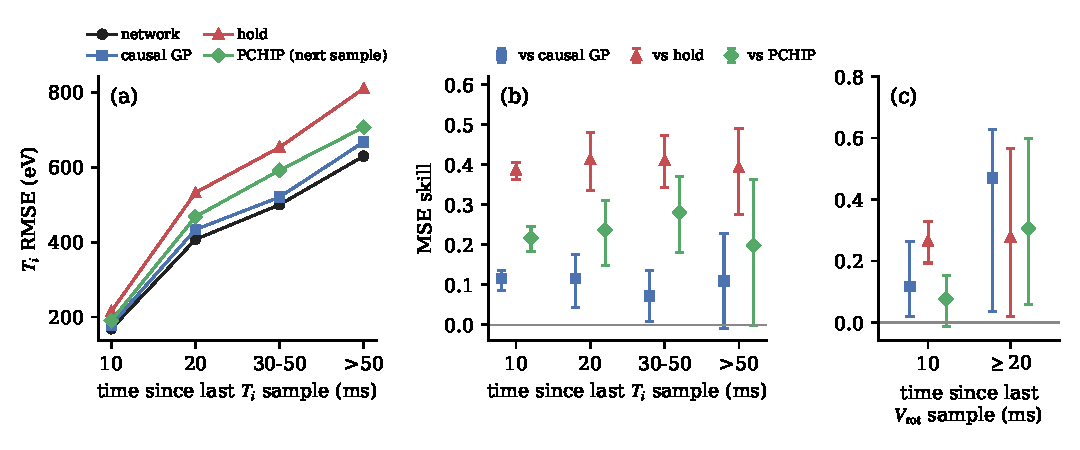
\includegraphics[width=\linewidth]{fig_gap}
  \caption{KSTAR, cut population: error against the time since the last observed CES
  value of the target (descriptive; pooled over the repeated cross-validation, so the
  RMSE level differs from the single split of Table~\ref{tab:ladder}). (a) \Ti{} RMSE
  of four estimators. (b) Mean-squared-error skill of the recurrent estimator for
  \Ti{} against three references, with 95\% intervals. (c) The same for \Vrot{} under
  the 1{,}000\,km/s scoring rule. 97.4\% of scored \Ti{} rows and 99.1\% of scored
  \Vrot{} rows are in the 10\,ms bin.}
  \label{fig:gap}
\end{figure}

\paragraph{Dependence on the gap.} Figure~\ref{fig:gap} resolves the same rows by the
time since the last observed value. This reading was not registered and is
descriptive. Every estimator has a larger error after a longer gap (\Ti{} RMSE of the
recurrent estimator 168.8\,eV at 10\,ms and 629.8\,eV beyond 50\,ms), which is the
other face of the missingness not being at random: gaps occur where the plasma is
changing. The skill over the causal GP does not shrink with the gap: $+0.115$
$[+0.085, +0.136]$ at 10\,ms, $+0.115$ $[+0.044, +0.176]$ at 20\,ms and $+0.072$
$[+0.008, +0.135]$ at 30--50\,ms, each interval excluding zero; beyond 50\,ms (464 to
505 rows per repeat) it is $+0.109$ $[-0.009, +0.228]$ and the interval includes zero.
In the inclusive population the 10\,ms and 30--50\,ms bins exclude zero ($+0.128$
$[+0.076, +0.176]$ and $+0.131$ $[+0.057, +0.202]$), while the 20\,ms bin ($+0.088$
$[-0.014, +0.214]$) and the bin beyond 50\,ms ($-0.003$ $[-0.127, +0.088]$) include it.
The margin is therefore not confined to rows adjacent to an observation, but the
long-gap bins are small, their intervals are wide, and the reading is weaker when
failed fits are kept.

\begin{table}[t]
  \centering
  \caption{KSTAR, \Ti{}: the recurrent estimator against the same network retrained
  with a \Ti{} branch that reads the CES history only (347{,}970 parameters; the fast
  channels are absent from its input, not zeroed), on the same test rows. Skill with
  discharge-clustered 95\% intervals on the four file-level splits; bold = interval
  excludes zero. In the cut population the history-only network stopped at the
  30-epoch cap on three of four splits (see text).}
  \label{tab:honly}
  \footnotesize
  \setlength{\tabcolsep}{4pt}
  \begin{tabular}{llccc}
    \toprule
    Population & Split & Full over history-only & History-only over causal GP & Full over causal GP \\
    \midrule
    \multirow{4}{*}{Cut}
      & 1 & $\mathbf{+0.067}$ $[+0.029, +0.108]$ & $+0.011$ $[-0.028, +0.047]$ & $\mathbf{+0.078}$ $[+0.035, +0.116]$ \\
      & 2 & $\mathbf{+0.077}$ $[+0.047, +0.106]$ & $\mathbf{+0.061}$ $[+0.030, +0.091]$ & $\mathbf{+0.133}$ $[+0.100, +0.163]$ \\
      & 3 & $\mathbf{+0.117}$ $[+0.093, +0.142]$ & $+0.024$ $[-0.005, +0.050]$ & $\mathbf{+0.138}$ $[+0.101, +0.175]$ \\
      & 4 & $\mathbf{+0.059}$ $[+0.011, +0.103]$ & $\mathbf{+0.049}$ $[+0.021, +0.076]$ & $\mathbf{+0.105}$ $[+0.056, +0.149]$ \\
    \midrule
    \multirow{4}{*}{Inclusive}
      & 1 & $+0.024$ $[-0.014, +0.057]$ & $\mathbf{+0.133}$ $[+0.025, +0.244]$ & $\mathbf{+0.154}$ $[+0.055, +0.262]$ \\
      & 2 & $+0.016$ $[-0.008, +0.033]$ & $\mathbf{+0.155}$ $[+0.080, +0.245]$ & $\mathbf{+0.169}$ $[+0.093, +0.253]$ \\
      & 3 & $\mathbf{+0.024}$ $[+0.012, +0.039]$ & $\mathbf{+0.102}$ $[+0.051, +0.155]$ & $\mathbf{+0.123}$ $[+0.073, +0.179]$ \\
      & 4 & $\mathbf{+0.023}$ $[+0.005, +0.053]$ & $\mathbf{+0.129}$ $[+0.043, +0.203]$ & $\mathbf{+0.149}$ $[+0.082, +0.218]$ \\
    \bottomrule
  \end{tabular}
\end{table}

\paragraph{How much of the margin is due to the fast channels?} The comparison above
is between a full-input estimator and CES-only estimators, and the margin could come
from the fast channels or from a better use of the CES past. The direct measurement is
the same network retrained with a \Ti{} branch that reads the CES history only, scored
on the same rows (Table~\ref{tab:honly}). The rule fixed before these runs was that
the fast-channel share is claimed if the interval of the full network's skill over
the history-only one lies above zero on at least three of the four cut splits. It
does on four of four ($+0.059$ to $+0.117$; the range written down beforehand was
$+0.05$ to $+0.14$). In the inclusive population the increment is $+0.016$ to $+0.024$
and its interval excludes zero on two of four splits, so the statement is conditional
on the cut population. The two populations also differ in where the margin over the
causal GP comes from. With failed fits excluded, the history-only network is
separated from the causal GP on two of four splits ($+0.011$ to $+0.061$), and the
margin of the full network over the causal GP ($+0.078$ to $+0.138$) is largely the
fast-channel increment. With failed fits kept, the history-only network alone has
$+0.102$ to $+0.155$ over the causal GP on four of four splits, and the fast channels
add little: there the margin comes mainly from how the recurrent state handles a CES
history that contains failed fits.
% B29-CAP-SLOT: replace the caveat below when the longer-cap rerun of the history-only
% network on the cut splits is read.

One caveat is open. In the cut population the history-only network was still
improving when training stopped at the cap of 30 epochs on three of the four splits
(best epoch 29, 30 and 30), whereas the full network reached that cap on one. An
undertrained history-only network would overstate the increment. The cap is the one
fixed in advance, and a rerun with a longer cap is not reported here
(\S\ref{sec:limits}). Four indirect measurements are consistent with a fast-channel
contribution in the cut population.
\begin{enumerate}
\item \emph{Sequence memory matters.} A memoryless regression (gradient-boosted trees)
on the same 22 inputs of the target row, including the last CES value, has a larger
error: the recurrent estimator's skill over it is $+0.156$ to $+0.231$ on the four cut
splits and $+0.104$ to $+0.180$ on the inclusive ones, every interval excluding zero.
That regression does not reach the causal GP (its interval against it includes zero or
lies below it on all four cut splits). One row of fast channels plus one CES value is therefore
not enough; the mainstream memoryless design of cross-diagnostic reconstruction would
not have found the margin.
\item \emph{A CES-only smoother explains part of the margin over interpolation.} Of
the skill over PCHIP on the first cut split ($+0.174$), a validation-tuned running
mean of the CES past already provides $+0.050$; the recurrent estimator's increment
over that running mean is $+0.113$ to $+0.137$ on the four cut splits, every interval
excluding zero.
\item \emph{Inside a 20-parameter filter, the fast-channel term is a measured
increment in the cut population.} The surrogate of \S\ref{sec:character:surrogate} is
a CES-only filter plus a linear fast-channel term. Against the same filter refitted with the
fast-channel gains set to zero, the full filter has skill $+0.037$ to $+0.070$ on the
four cut splits
(every interval excluding zero), which is 0.34--0.58 of the recurrent estimator's
margin over that CES-only filter ($+0.109$ to $+0.130$). In the inclusive population
the increment is not resolved (0 of 4 splits).
\item \emph{The association exists at the level of increments.} Corrected for target
noise, the correlation between fast-channel increments and \Ti{} increments has a 95\%
lower bound of at least $+0.127$ at zero lag for every window between 10 and 200\,ms.
\end{enumerate}
These bound the fast-channel share from below within a linear filter and show that
memory is necessary. Together with Table~\ref{tab:honly} the \Ti{} result is: a
full-input estimator that does not use the next CES sample has a lower error than
CES-only estimators of that kind; with failed fits excluded, most of its margin over
the causal GP is lost when the fast channels are removed from the network, subject to
the open check on training length; with failed fits kept, the fast-channel share is
small.

\paragraph{What the fast channels are responding to.} The response of the trained
network to the fast channels is a same-instant co-movement: its Jacobian is a
high-pass kernel of about 100\,ms (the current value minus the mean of the preceding
ten steps), flat to about two standard deviations and switched off beyond three.
Truncating the network's context costs $-0.066$ in skill at 20\,ms and saturates at
50\,ms. The autocorrelation $1/e$ times of \Ti{} (159\,ms), BES (161\,ms) and ECEI
(147\,ms) agree, as expected if the three follow the same local evolution. The physical
mechanism is not identified: per-discharge standardization removes the absolute $T_e$
and $n_e$ that the exchange term of~\eqref{eq:energy} would need, and the files carry
no beam-power or D-alpha signal with which events could be labelled. At 10\,ms no
statement about individual ELMs is possible.

\subsection{Rotation}
\label{sec:fast:vrot}

\paragraph{A bound on the coupling.} Corrected for target noise, the correlation of
fast-channel increments with \Vrot{} increments has a 95\% bound $|r| \leq 0.044$ over
every lag from 0 to 200\,ms and every window from 10 to 200\,ms, against the \Ti{}
lower bound of $+0.127$. This bounds a linear association and does not prove its
absence (BES at 100--200\,ms gives $r \approx +0.01$ with an interval excluding zero).
It is the measured counterpart of the asymmetry between~\eqref{eq:energy}
and~\eqref{eq:momentum}. Two further routes to rotation information were examined. The
Mirnov signal at 100\,Hz equals a single raw sample of the 2\,MHz stream at the grid
time on 24 of 24 coils checked, a point snapshot, so mode rotation in the kHz band
(edge harmonic oscillations near 4 and 8\,kHz occur in this data set) is aliased away;
its lag-1 autocorrelation is $-0.009$ against $+0.568$ for BES. No torque or beam-power
channel exists, so the beam-torque route is untested. The statement is scoped to
standard CES at 10\,ms on the $R = 2.198$\,m chord; edge rotation inside an ELM
cycle~\citep{Viezzer2020Dynamics} is a different measurement.

\paragraph{The history-only estimate.} Rotation is estimated by the branch that reads
the CES past only (Table~\ref{tab:headline}, \Vrot{} block). Removing the fast
channels from the \Ti{} branch leaves the rotation error where it was (skill of the
full network over the retrained one $-0.005$ to $+0.010$, no interval excluding zero
in either population), as the wiring implies. Among estimators that do
not use the next CES sample this branch has the lowest mean squared error
(Table~\ref{tab:ladder}). Its skill over persistence is $+0.265$ $[+0.198, +0.326]$
(cut), with the interval excluding zero on all four splits in both populations, and
the same holds over a validation-tuned running mean of the rotation past, so the
estimate is not reducible to a running mean. Over the causal GP the pooled interval
excludes zero in both populations; per split the point estimates are all positive
($+0.057$ to $+0.131$, cut) but the interval excludes zero on 1 of 4 cut splits and 2
of 4 inclusive ones, so that margin is established in the pooled readout only. Against
PCHIP, which uses the following sample, the interval excludes zero in the cut
population by a narrow margin and includes zero in the inclusive one and at
thresholds of 500 and 2{,}000\,km/s, so a margin over PCHIP is not established.
Against the offline GP the offline smoother has the lower error in the inclusive
population. Resolved by gap (Fig.~\ref{fig:gap}c), the 653 to 677 rows per repeat that
follow a gap of 20\,ms or more show skill $+0.470$ $[+0.036, +0.628]$ over the causal
GP and $+0.305$ $[+0.059, +0.598]$ over PCHIP, with wide intervals.

\paragraph{The scoring rule.} All rotation numbers are under a scoring rule that drops,
from every estimator, the 36--41 rows per repeat (0.05\%) whose target or anchor
exceeds $|\Vrot| = 1{,}000$\,km/s. The rule was set after a first analysis without it
had been seen; that analysis and the reason for the rule are in
Appendix~\ref{app:vrotrule}.

\subsection{Two stress tests}
\label{sec:fast:stress}
\emph{Missingness not at random.} Reweighting the scored rows onto the covariate
distribution (time since the last observation and local activity) of the rows that are
actually missing and inside the scored domain, 53.6--67.0\% (cut) of the missing
\Ti{} rows, gives \Ti{} skill over PCHIP of $+0.14$ to $+0.28$, with intervals
excluding zero on 2 of 4 cut and 4 of 4 inclusive splits, and over persistence
$+0.28$ to $+0.44$ with intervals excluding zero in all eight cells. Missing \Vrot{}
rows are only 4--6\% inside the scored domain and nothing is concluded for them.
\emph{Later discharges.} With a strictly temporal split (train on 416 shots, validate
on 128, test on the 97 latest), the \Ti{} skill is $+0.17$ to $+0.20$ over PCHIP and
$+0.11$ to $+0.16$ over the causal GP, with intervals excluding zero for all four
initialisations in both populations; for \Vrot{} it is $+0.33$ over persistence (cut,
four of four). The fast diagnostics drift by 1.22 (BES) and 0.53 (ECEI) standard
deviations between the two periods against 0.115 for the targets. Per-discharge
standardization, which absorbs that drift, was adopted after an earlier design failed
this split and it uses whole-discharge statistics, so this is not an independent test
of a deployable estimator.

% =========================================================================
\section{The character of the gain}
\label{sec:character}

\subsection{Mean and median}
\label{sec:character:median}
A mean-squared-error skill is decided by few rows. On KSTAR the 1\% of rows with the
largest squared \Ti{} error of the recurrent estimator carry 48\% (cut) and 83\%
(inclusive) of its total. On a typical row the estimator carries its last value: its
median absolute \Ti{} error, 47.2\,eV, is close to that of persistence (46.1\,eV) and
to the 10\,ms scatter of the target (46.4\,eV), while PCHIP reaches 39.4\,eV by
averaging with the following sample (median-absolute-error skill $-0.198$
$[-0.259, -0.135]$). The ratio of the estimator's error to PCHIP's falls below 1 only
in the upper error quartile. For rotation the median row is worse than persistence
(4.3 against 3.7\,km/s; median-absolute-error skill against PCHIP $-0.488$ cut and
$-0.518$ inclusive, interval below zero on all four splits). The aggregate skill is
thus a deficit on the bulk offset by a gain on the tail. Under a symmetric 1\% trim
and under a Huber loss at the noise bound the \Ti{} skill over PCHIP stays $+0.210$ and
$+0.156$ (cut, both intervals excluding zero); the inclusive trimmed skill is $+0.057$
with an interval including zero.

The same character appears on MAST without any network: the mean-to-median ratio of
\chir{} of the best CES-only estimator is 6 to 7, about three times the Gaussian value
(\S\ref{sec:floor:mast}). In both regimes the typical hidden sample is already estimated
to within its fit noise by the simplest reference, and what an estimator can add is
concentrated in the rows where the plasma moved. This is why link (B) matters for
link (D): in a noise-limited regime the median row leaves nothing to gain, and a
fast-diagnostic term can only act on events.

\subsection{A 20-parameter reading of the ion-temperature branch}
\label{sec:character:surrogate}
The weights of the trained networks carry no stable reading (first-layer column norms
are flat across the fifteen fast channels and per-channel ranks do not reproduce
across splits), but the input--output response does. Read from the response, the
\Ti{} output is an exponentially weighted average of past observed \Ti{} plus the
high-pass fast-channel response described in \S\ref{sec:fast:ti}. Written as a filter
and trained from scratch under the identical protocol:
\begin{gather}
  \hat y_t = m_t + \sum_{c=1}^{15} a_c\, d_{c,t}\,
     \sigma\!\Bigl(\frac{\theta-|d_{c,t}|}{0.5}\Bigr) + b_0,
  \qquad
  d_{c,t} = x_{c,t} - \overline{x}_{c,\,t-10..t-1},
  \label{eq:surrogate}\\
  m_t = m_{t-1} + K(s)\,(y^\mathrm{obs} - m_{t-1}),
  \qquad
  K(s) = K_\infty + (K_0 - K_\infty)\,e^{-s/s_K},
  \label{eq:gain}
\end{gather}
where $m_t$ is updated only when a new \Ti{} measurement arrives, $s$ is the time
since the previous one, $\sigma(\cdot)$ is the logistic function, and $d_{c,t}$ and
$\theta$ are in per-discharge standard deviations. Its 20 parameters are three gain
constants, one gain $a_c$ per fast channel, the threshold $\theta$ and the offset
$b_0$. On the four cut splits the learned values are $K_0 = 0.27$--$0.30$,
$K_\infty = 0.48$--$0.53$, $s_K = 39$--$47$\,ms, $\theta = 2.9$--$3.0$ standard
deviations, and summed gains of $+48$ to $+53$\,eV per standard deviation for BES and
$+44$ to $+50$ for ECEI.

This filter keeps 72--78\% of the recurrent estimator's skill over PCHIP and 87--90\%
of its skill over persistence on the four cut splits; measured against the causal GP
it keeps 0.31 to 0.50. Three qualifications bound what it shows. The form of the
fast-channel term was read from the network's Jacobian on the test rows of the same
four splits on which the filter is scored, so the retention is post hoc. It holds in
the cut population only (0.43--0.81 inclusive, where the BES gain changes sign under
the fit-failure spikes). And as a standalone estimator the filter has skill $+0.02$ to
$+0.07$ over the causal GP with the interval excluding zero on 2 of 4 cut splits, and
is below the offline GP on all four; it is an interpretation of the network, not a
replacement for it. The remaining 22--28\% is nonlinear event handling that the forms
tried here do not reproduce.

\paragraph{What the gain $K(s)$ does and does not mean.} In the jointly trained filter
the gain rises with the gap, from $K_0$ for a fresh measurement to $K_\infty$ after a
long one, which reads like a Kalman update that trusts a new CES sample more the longer
it has waited. That reading does not survive a control. When the same filter is refit
with every fast-channel gain set to zero, a 4-parameter CES-only filter, the optimal
gain is flat or falls with the gap: 0.30--0.32 at 10\,ms, 0.24--0.27 at 20\,ms and
0.23--0.26 at 50\,ms (cut). The rising gain is therefore a property of the joint fit
with the fast-channel term and not of the CES series alone; in the joint fit the
fast-channel term carries the recent change, and the CES update is free to weight a
late sample more.

% =========================================================================
\section{Limitations}
\label{sec:limits}

\begin{itemize}
\item \emph{The fast-channel share of the \Ti{} margin is conditional and carries an
open check.} It is established in the cut population (four of four splits) and is
small in the inclusive one (two of four). In the cut population the history-only
network stopped at the 30-epoch cap on three of four splits, so it may be
undertrained and the increment overstated; a rerun with a longer cap is not reported
here.
% B29-CAP-SLOT (limitations 1): rewrite when the longer-cap rerun is read.
\item \emph{The estimator is not causal as trained.} The fast channels are
standardized with whole-discharge statistics. Variants with train-file statistics and
with a standardizer that uses past rows only are not reported here, nor is a
memoryless network on the same inputs; whether the margin over the causal GP survives
a past-only standardizer is not known under this protocol. The estimator is therefore
described as one that does not use the next CES sample, not as a causal one.
% B29-SLOT (limitations 2): arms B/C (train-file and expanding-window standardizers), arm D.
\item \emph{Tail statistic.} The skill is carried by large-error rows; typical rows
are not improved over interpolation (\S\ref{sec:character:median}).
\item \emph{Post hoc choices.} The 1{,}000\,km/s rotation scoring rule and the form of
the 20-parameter filter were chosen after results were seen; both are labelled where
used. The recurrent design and per-discharge standardization were adopted using the
same four test splits.
\item \emph{Scope on KSTAR.} One chord, one campaign, one device. The normalized
radius of the chord (0.80) is from nominal geometry, not from an equilibrium, and the
files carry no confinement-mode label, so whether the chord sits at the pedestal top
or inside it in a given discharge is not established; the motivation from a weak
edge-side signal rests on the temperature level at the chord, on the missingness and
on the MAST radial breakdown. The per-discharge relation between the regime number and
the estimator ordering is computed from the rows that are scored, inside a
noise-dominated range. There is no per-exposure fit uncertainty, so fit failures are
handled by value rules;
there is no beam-power, D-alpha or equilibrium signal, so no event is labelled and no
transport quantity is derived.
\item \emph{Scope on MAST.} Gaps are made by hiding frames; the reported errors are
taken as stored, and for \Vi{} they are smaller than the frame-to-frame scatter; one
hyperparameter remains on a grid edge; the causal-GP window is fixed at eight frames;
the paired difference between the causal GP and the slope-state filter was not
bootstrapped. No learned estimator and no fast diagnostic was used on MAST. The
breakdowns by campaign, array layout and normalized radius were made after the pooled
result was known, over many strata, without correction for multiple comparisons; the
strata are confounded with each other; the normalized radius uses one axis and one
boundary radius per discharge; the bin of the KSTAR radius holds 26 shots under the
primary fit rule; and the reported \Ti{} errors are scaled differently from campaign
to campaign.
\item \emph{Intervals.} The unit of replication is the discharge. The pooled KSTAR
interval conditions on the trained models; the fold-level interval, which does not,
is wider and for rotation against the causal GP was not computed under the scoring
rule.
\end{itemize}

% =========================================================================
\section{Conclusion}
\label{sec:conclusion}

How well a missing charge-exchange sample can be estimated without the next one is set
first by the regime of the series, and the regime follows the strength of the
measurement. On the edge-side KSTAR chord at 10\,ms the increments of \Ti{} and
\Vrot{} are close to white fit noise (lag-1 autocorrelation $-0.416$ and $-0.349$),
averaging the CES past helps, and CES-only estimators saturate near a causal GP;
from discharge to discharge the same number orders the running mean and the causal
GP (rank correlation $+0.338$ $[+0.213, +0.451]$ for \Ti{}). On MAST the increments
pooled over radius are trend-dominated ($+0.297$ and $+0.463$) and averaging does not
help, but the fit rule fails 0.430 of the samples at the normalized radius of the
KSTAR chord against 0.231 in the core, and there the \Ti{} number, $+0.103$
$[-0.079, +0.257]$, is not separated from zero. The best CES-only estimator of that
kind leaves a mean residual of 2.57 $[1.94, 3.40]$ (\Ti{}) and 16.69 $[12.96, 21.04]$
(\Vi{}) times what the reported fit errors predict, most of it in a tail; for \Ti{}
this holds in two of the four campaigns.

The main result is on KSTAR. Among estimators that do not use the next CES sample, an
estimator that also reads BES and ECEI channels at the location of the chord has the
lowest mean squared error for \Ti{}, with skill $+0.113$ $[+0.085, +0.132]$ over the
CES-only causal GP; against an offline GP that uses the next sample the interval
includes zero. The same network retrained without the fast channels has a larger
error by $+0.059$ to $+0.117$ on the four splits when failed fits are excluded, which
is most of the margin over the causal GP, and by $+0.016$ to $+0.024$ when they are
kept; the first figure awaits a check on training length. Rotation shows a bounded
association with the same channels ($|r| \leq 0.044$) and is estimated from its own
history, with skill $+0.265$ $[+0.198, +0.326]$ over persistence and $+0.121$
$[+0.074, +0.187]$ over a running mean. In both cases the gain belongs to the rows
where the plasma moved, and a 20-parameter filter reproduces most of the \Ti{} part.

The measurements that would change these statements are named: a longer-trained
history-only network and the causally standardized variants (\S\ref{sec:limits}); an
equilibrium mapping and per-exposure fit uncertainties for the KSTAR chord, which
would place it relative to the pedestal and give its noise floor; and additional
KSTAR chords, on which the MAST radial breakdown predicts a less noise-dominated
series inward of the present one.

\section*{Data and code availability}
The MAST data are public (FAIR-MAST, CC BY-SA 4.0); the shot lists, the registration
documents, the analysis code and all evaluation artifacts are at
\url{https://github.com/iseungsang01/ml-intern-revision}. The KSTAR shot files are not
redistributable. [TO BE COMPLETED BY AUTHORS: data-access statement for KSTAR.]

\section*{Acknowledgments}
[TO BE COMPLETED BY AUTHORS: data provider and permission for the KSTAR 2022 CES, BES,
ECEI and Mirnov data; funding; co-authorship and affiliations.]

% =========================================================================
\appendix

\section{Registration history and order of events}
\label{app:registration}

\paragraph{KSTAR.} Test files were reserved before the architecture was chosen. The
adoption of the full-grid recurrent design and of per-discharge standardization used
results on the same four test splits, and the repeated cross-validation re-partitions
the same discharges. The form of the 20-parameter filter was read from the response of
the trained network on those test rows. The rotation scoring rule was set after a
first analysis (Appendix~\ref{app:vrotrule}). The regime number of
\S\ref{sec:regime} and the gap-resolved reading of Fig.~\ref{fig:gap} were computed for
this paper and were not registered. The per-discharge relation between the regime
number and the estimator ordering (Table~\ref{tab:tertile}) was registered, with both
predictions and the minimum of 30 scored rows per discharge, after the distribution of
the regime number was known and before any per-discharge skill was computed. The
history-only network (Table~\ref{tab:honly}) was registered with its decision rule
before it was trained; it is one of four registered variants and the only one run so
far, its training batch was interrupted and resumed from saved runs, and the epoch
cap was the registered one.

\paragraph{MAST.} In order: (i) a pilot of 13 shots was inspected and those shots were
excluded; (ii) the list of 300 shots, the fit rule, the tuning/test division, the
estimators, the independence test and both decision rules were committed before any
value of the 300 shots was read; (iii) the first run was executed. During it the
stored frame times of a few shots were found to be irregular or non-increasing, which
produced negative time steps in the slope-state filter; the nominal 5\,ms grid was
adopted after a first test-set table had been seen. Both decisions were the same
before and after that change, and dropping the affected shots (4 in population G) changes
neither. (iv) Several tuned hyperparameters of the first run sat on the edge of their
grid, so a second run with wider grids and a stopping rule (extend an edge-bound grid
at most twice more) was registered before it was computed, with the first run kept on
record. (v) In the second run the \Vi{} tuning was at first started from the grids on
which the \Ti{} tuning had ended, which was not the registered procedure; it was
rerun from the registered grids. The \Ti{} numbers are identical in the two
executions; for \Vi{} only the offline-GP selection differs. One hyperparameter (the
offline-GP amplitude for \Vi{}) remains on an edge after the allowed extensions.
(vi) The breakdowns by campaign, heating, coil state, array layout and normalized
radius were made after the test-set result was known, without retuning. Their strata
and eight statements were written down before the stratified values were computed. Of
those eight, the positive regime number in every campaign, the running mean at or
below persistence in every campaign, and the positive \Vi{} regime number at the
KSTAR radius held; the \Ti{} residual above 1.5 in every campaign, the positive \Ti{}
regime number at the KSTAR radius under the primary fit rule, and the three
statements that asked for a monotone dependence on radius did not; the statement
that shots without a beam block concentrate among south-west-beam-only shots could
not be read as written, because those shots carry no arrays at all.

\section{The first registered MAST run}
\label{app:mastfirst}

Table~\ref{tab:mastfirst} gives the first registered run beside the run with wider
grids reported in the main text. In the first run the GP amplitude was limited to four
times the median reported error, which placed its optimum on the edge of the grid, and
the causal GP had a larger error than persistence; the slope-state filter was then the
best estimator that does not use the following sample. For \Ti{} the slope-state
filter was already at its optimum and does not move between the runs. The two
decisions are the same in both runs: the independence statistic does not depend on the
tuning, and the mean \chir{} of the best such estimator is 2.71 $[2.07, 3.51]$ (\Ti{})
and 21.20 $[16.83, 26.06]$ (\Vi{}) in the first run against 2.57 $[1.94, 3.40]$ and
16.69 $[12.96, 21.04]$ in the second, all four intervals above 1.5.

\begin{table}[h]
  \centering
  \caption{MAST test set, population G: skill over persistence in the first registered
  run and in the run with wider tuning grids. Estimators without a hyperparameter are
  identical in the two runs. Bold = interval excludes zero.}
  \label{tab:mastfirst}
  \footnotesize
  \setlength{\tabcolsep}{5pt}
  \begin{tabular}{llcc}
    \toprule
    Target & Estimator & First run & Wider grids \\
    \midrule
    \multirow{4}{*}{\Ti{}}
      & running mean & $\mathbf{-0.143}$ $[-0.189, -0.103]$ & $\mathbf{-0.012}$ $[-0.017, -0.007]$ \\
      & slope-state filter & $+0.076$ $[-0.006, +0.148]$ & $+0.076$ $[-0.006, +0.148]$ \\
      & causal GP & $\mathbf{-0.683}$ $[-0.997, -0.426]$ & $\mathbf{+0.136}$ $[+0.069, +0.208]$ \\
      & offline GP & $\mathbf{+0.374}$ $[+0.093, +0.568]$ & $\mathbf{+0.538}$ $[+0.425, +0.620]$ \\
    \midrule
    \multirow{4}{*}{\Vi{}}
      & running mean & $\mathbf{-0.232}$ $[-0.290, -0.179]$ & $\mathbf{-0.024}$ $[-0.030, -0.018]$ \\
      & slope-state filter & $\mathbf{+0.088}$ $[+0.035, +0.147]$ & $\mathbf{+0.108}$ $[+0.049, +0.175]$ \\
      & causal GP & $\mathbf{-0.350}$ $[-0.499, -0.238]$ & $\mathbf{+0.110}$ $[+0.055, +0.168]$ \\
      & offline GP & $\mathbf{+0.577}$ $[+0.435, +0.696]$ & $\mathbf{+0.622}$ $[+0.498, +0.727]$ \\
    \bottomrule
  \end{tabular}
\end{table}

\section{The rotation scoring rule}
\label{app:vrotrule}

As first registered, without any rule for rotation fit failures, the pooled skill of
the rotation branch over PCHIP was $+0.313$ $[+0.072, +0.701]$. That interval rested on
36--41 of about 71{,}700 rows per repeat (0.05\%) whose target, persistence anchor or
PCHIP anchor exceeds $|\Vrot| = 1{,}000$\,km/s; those rows carry 63--78\% of PCHIP's
squared error. The rule that removes them from every estimator was set after that
first analysis, once their share was known, and is applied at scoring only: the
history inputs still contain those values and no model was retrained. Under the rule
the pooled skill over PCHIP is $+0.092$ $[+0.0003, +0.170]$ (cut) and $+0.090$
$[-0.010, +0.177]$ (inclusive), and it includes zero in both populations at thresholds
of 500 and 2{,}000\,km/s. All rotation numbers in this paper are under the rule; the
registered value without it is reported here for the record and is not used.

\bibliographystyle{unsrtnat}
\bibliography{refs}

\end{document}
